% RepNet Progress Update — Finalized Model Performance
% Same visual identity as final_presentation_modern.tex
% Compiles with pdfLaTeX.

\documentclass[10pt,aspectratio=169]{beamer}

% ====================
% Packages
% ====================
\usepackage[T1]{fontenc}
\usepackage{lmodern}
\usepackage{graphicx}
\usepackage{booktabs}
\usepackage{mathtools}
\usepackage{tikz}
\usepackage{hyperref}
\usepackage{pgfplots}
\pgfplotsset{compat=1.18}
\usepgfplotslibrary{groupplots}
\pgfmathdeclarefunction{ecgbeat}{1}{%
  \pgfmathparse{%
    0.15*exp(-((#1-0.16)^2)/0.0032)%
    -0.08*exp(-((#1-0.32)^2)/0.000288)%
    +1.0*exp(-((#1-0.36)^2)/0.0002)%
    -0.2*exp(-((#1-0.4)^2)/0.00045)%
    +0.25*exp(-((#1-0.55)^2)/0.0032)%
  }%
}
\pgfmathdeclarefunction{ecgsig}{1}{%
  \pgfmathparse{ecgbeat(#1)+ecgbeat(#1-0.8)}%
}

% ====================
% UC Davis brand colors (digital palette)
% ====================
\definecolor{aggieblue}{HTML}{022851}
\definecolor{aggiegold}{HTML}{FFBF00}
\definecolor{aggieblueDark}{HTML}{011936}
\definecolor{aggiegoldDark}{HTML}{C99700}
\definecolor{coolgray}{RGB}{77,79,83}
\definecolor{boxgray}{RGB}{238,235,233}

% ====================
% Fonts
% ====================
\renewcommand{\familydefault}{\sfdefault}
\newcommand{\Raleway}{\sffamily}
\newcommand{\Lato}{\sffamily}

% ====================
% Beamer color slots
% ====================
\setbeamercolor*{palette primary}{fg=white,bg=aggieblue}
\setbeamercolor*{palette secondary}{fg=white,bg=coolgray}
\setbeamercolor*{palette tertiary}{fg=white,bg=aggieblueDark}
\setbeamercolor*{palette quaternary}{fg=aggieblue,bg=aggiegold}

\setbeamercolor{structure}{fg=aggieblue}
\setbeamercolor{titlelike}{fg=aggieblue}
\setbeamercolor{frametitle}{fg=white,bg=aggieblue}
\setbeamercolor{title}{fg=white,bg=aggieblue}
\setbeamercolor{author}{fg=aggieblue}
\setbeamercolor{institute}{fg=coolgray}
\setbeamercolor{date}{fg=coolgray}

\setbeamercolor{itemize item}{fg=aggieblue}
\setbeamercolor{itemize subitem}{fg=aggiegoldDark}
\setbeamercolor{enumerate item}{fg=aggieblue}
\setbeamercolor{description item}{fg=aggieblue}

\setbeamercolor{block title}{fg=white,bg=aggieblue}
\setbeamercolor{block body}{fg=black,bg=boxgray}
\setbeamercolor{block title alerted}{fg=aggieblue,bg=aggiegold}
\setbeamercolor{block body alerted}{fg=black,bg=boxgray}

\setbeamercolor{section in toc}{fg=aggieblue}
\setbeamercolor{subsection in toc}{fg=aggieblueDark}
\setbeamercolor{caption name}{fg=aggieblue}

% ====================
% Fonts (sizes/weights)
% ====================
\setbeamerfont{title}{family=\Raleway,series=\bfseries,size=\LARGE}
\setbeamerfont{subtitle}{family=\Lato,size=\normalsize}
\setbeamerfont{author}{family=\Lato,size=\small}
\setbeamerfont{institute}{family=\Lato,size=\footnotesize}
\setbeamerfont{date}{family=\Lato,size=\footnotesize}
\setbeamerfont{frametitle}{family=\Raleway,series=\bfseries,size=\large}
\setbeamerfont{block title}{family=\Raleway,series=\bfseries}
\setbeamerfont{section in toc}{family=\Raleway,series=\bfseries}
\setbeamerfont{footline}{family=\Lato,size=\scriptsize}

% ====================
% Frame title with Aggie Gold accent bar
% ====================
\setbeamertemplate{frametitle}{%
  \nointerlineskip
  \begin{beamercolorbox}[wd=\paperwidth,ht=3.0ex,dp=1.4ex,leftskip=1em,rightskip=1em]{frametitle}%
    \usebeamerfont{frametitle}\insertframetitle%
  \end{beamercolorbox}%
  \begin{beamercolorbox}[wd=\paperwidth,ht=0.35ex,dp=0pt]{palette quaternary}%
  \end{beamercolorbox}%
  \vspace{1.0ex}
}

\beamertemplatenavigationsymbolsempty

% ====================
% Itemize bullet
% ====================
\setbeamertemplate{itemize item}{\raise0.5ex \hbox{\vrule width 0.5ex height 0.5ex}}
\setbeamertemplate{itemize subitem}{\raise0.3ex \hbox{\vrule width 0.5ex height 0.5ex}}
\setbeamertemplate{itemize subsubitem}{\raise0.2ex \hbox{\vrule width 0.5ex height 0.5ex}}

% ====================
% Footer
% ====================
\newcommand{\footercontent}[1]{\renewcommand{\insertfootercontent}{#1}}
\newcommand{\insertfootercontent}{}

\setbeamertemplate{footline}{%
  \ifx\insertfootercontent\@empty\else
    \begin{beamercolorbox}[wd=\paperwidth,ht=0.3ex,dp=0pt]{palette quaternary}\end{beamercolorbox}%
    \begin{beamercolorbox}[wd=\paperwidth,ht=2.4ex,dp=1.2ex,leftskip=1em,rightskip=1em]{palette primary}%
      \usebeamerfont{footline}\insertfootercontent\hfill\insertframenumber{}/\inserttotalframenumber%
    \end{beamercolorbox}%
  \fi
}

% ====================
% Section divider slide
% ====================
\AtBeginSection[]{%
  \begin{frame}[plain,noframenumbering]
    \begin{tikzpicture}[remember picture,overlay]
      \fill[aggieblue] (current page.south west) rectangle (current page.north east);
      \fill[aggiegold] ([yshift=-0.6cm]current page.center) rectangle ([yshift=-0.55cm,xshift=4cm]current page.center);
      \fill[aggiegold] ([yshift=-0.6cm]current page.center) rectangle ([yshift=-0.55cm,xshift=-4cm]current page.center);
      \node[anchor=center,text=white,font=\Raleway\bfseries\Huge]
        at ([yshift=0.4cm]current page.center) {\insertsectionhead};
    \end{tikzpicture}
  \end{frame}
}

% ====================
% pgfplots common styles
% ====================
\pgfplotsset{
    repnet base/.style={
        grid=none,
        tick label style={font=\tiny},
        label style={font=\scriptsize},
    },
    optim history/.style={
        repnet base,
        width=7.2cm,
        height=5.0cm,
        xlabel={Trial},
        ylabel={CV AUROC},
        ymin=0.64, ymax=0.71,
    },
}

% ====================
% Title / authors
% ====================
\title{RepNet Progress Update}
\subtitle{Finalized Model Performance}
\author{Ahmed Khan \and Lawrencedel Legaspi \and Selena Phu}
\institute{Department of Electrical and Computer Engineering \\ University of California, Davis}
\date{\today}

\titlegraphic{
\includegraphics[height=2.0cm]{logo.png}}

\footercontent{%
  \href{https://github.com/AhmedKhan-GH/repnet}{github.com/AhmedKhan-GH/repnet}
  \enspace$\bullet$\enspace
  UC Davis Senior Design 2026
  \enspace$\bullet$\enspace
  \href{mailto:aekhan@ucdavis.edu}{aekhan@ucdavis.edu}%
}

% ====================
% Title page template
% ====================
\setbeamertemplate{title page}{%
  \begin{tikzpicture}[remember picture,overlay]
    \fill[aggieblue]
      ([yshift=1cm]current page.north west)
      rectangle
      ([yshift=-3.8cm]current page.north east);
    \fill[aggiegold]
      ([yshift=-3.8cm]current page.north west)
      rectangle
      ([yshift=-3.95cm]current page.north east);
    \node[anchor=center,text=white,align=center,text width=14cm,
          font=\Raleway\bfseries]
      at ([yshift=-1.6cm]current page.north)
      {\usebeamerfont{title}\inserttitle};
    \node[anchor=center,text=aggiegold,align=center,text width=14cm,
          font=\Lato]
      at ([yshift=-2.4cm]current page.north)
      {\usebeamerfont{subtitle}\insertsubtitle};
    \node[anchor=north]
      at ([yshift=-4.3cm]current page.north)
      {\inserttitlegraphic};
    \node[anchor=north,text=aggieblue,align=center,font=\Lato]
      at ([yshift=-6.5cm]current page.north)
      {\usebeamerfont{author}\insertauthor};
    \node[anchor=north,text=coolgray,align=center,font=\Lato]
      at ([yshift=-7.1cm]current page.north)
      {\usebeamerfont{institute}\insertinstitute};
    \node[anchor=north,text=coolgray,align=center,font=\Lato]
      at ([yshift=-8.0cm]current page.north)
      {\usebeamerfont{date}\insertdate};
  \end{tikzpicture}%
}

% ====================
% Document
% ====================
\begin{document}

% ---------- Title ----------
{%
  \setbeamertemplate{footline}{}%
  \begin{frame}[plain,noframenumbering]
    \titlepage
  \end{frame}
}

% ---------- TOC ----------
\begin{frame}{Contents}
  \tableofcontents
\end{frame}

% =========================================================
\section{Architecture}
% =========================================================

\begin{frame}{RepNet CrossLead --- 3-Stage Architecture}
  \centering
  \vspace{-0.3em}
  {\footnotesize\color{coolgray}%
   \textcolor{aggieblue}{\textbf{Per-lead convolution}} (channel independence)
   alternates with
   \textcolor{aggiegoldDark}{\textbf{cross-lead attention}} (information exchange)
   at three abstraction depths.}
  \vspace{0.4em}

  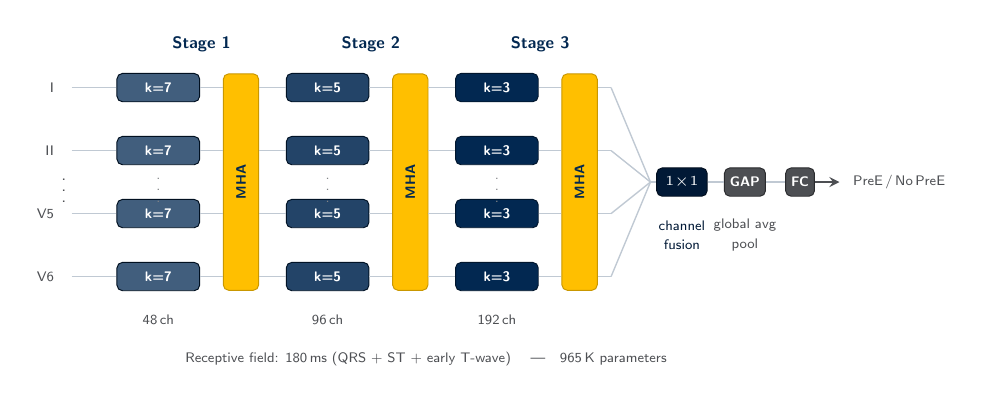
\begin{tikzpicture}[
    x=1cm, y=1cm,
    >=stealth,
    convA/.style={
      rectangle, rounded corners=2pt,
      minimum width=1.05cm, minimum height=0.36cm,
      fill=aggieblue!75, draw=aggieblue!40!black, line width=0.35pt,
      text=white, font=\fontsize{5}{6}\selectfont\bfseries,
      inner sep=1pt,
    },
    convB/.style={
      rectangle, rounded corners=2pt,
      minimum width=1.05cm, minimum height=0.36cm,
      fill=aggieblue!87, draw=aggieblue!47!black, line width=0.35pt,
      text=white, font=\fontsize{5}{6}\selectfont\bfseries,
      inner sep=1pt,
    },
    convC/.style={
      rectangle, rounded corners=2pt,
      minimum width=1.05cm, minimum height=0.36cm,
      fill=aggieblue, draw=aggieblue!55!black, line width=0.35pt,
      text=white, font=\fontsize{5}{6}\selectfont\bfseries,
      inner sep=1pt,
    },
    fusebox/.style={
      rectangle, rounded corners=2pt,
      minimum height=0.36cm,
      fill=aggieblueDark, draw=aggieblueDark!55!black, line width=0.35pt,
      text=white, font=\fontsize{5}{6}\selectfont\bfseries,
      inner sep=3pt,
    },
    headbox/.style={
      rectangle, rounded corners=2pt,
      minimum height=0.36cm,
      fill=coolgray, draw=coolgray!55!black, line width=0.35pt,
      text=white, font=\fontsize{5}{6}\selectfont\bfseries,
      inner sep=2pt,
    },
    attnbox/.style={
      rectangle, rounded corners=2pt,
      minimum width=0.45cm,
      fill=aggiegold, draw=aggiegoldDark, line width=0.35pt,
      text=aggieblue, font=\fontsize{4}{5}\selectfont\bfseries,
      inner sep=1pt,
    },
    wire/.style={draw=aggieblue!25, line width=0.5pt},
    annot/.style={font=\fontsize{4.5}{5.5}\selectfont, text=coolgray},
    stagelab/.style={font=\fontsize{6}{7}\selectfont\bfseries, text=aggieblue},
  ]

  % --- Lead labels + input wires ---
  \foreach \lid/\y/\name in {a/1.2/I, b/0.4/II, c/-0.4/V5, d/-1.2/V6} {
    \node[font=\fontsize{5}{6}\selectfont, text=coolgray, anchor=east]
      at (-0.1, \y) {\name};
    \draw[wire] (0, \y) -- (0.4, \y);
  }
  \node[font=\fontsize{6}{7}\selectfont, text=coolgray] at (-0.1, 0) {$\vdots$};

  % ================================================================
  %  STAGE 1  —  Conv k=7, 48 ch
  % ================================================================
  \foreach \lid/\y in {a/1.2, b/0.4, c/-0.4, d/-1.2} {
    \node[convA] (c1\lid) at (1.1, \y) {k=7};
    \draw[wire] (0.4, \y) -- (c1\lid.west);
    \draw[wire] (c1\lid.east) -- (1.85, \y);
  }
  \node[annot, text=coolgray!70] at (1.1, 0) {$\vdots$};
  % -- Attention block --
  \node[attnbox, minimum height=2.75cm] (a1) at (2.15, 0)
    {\rotatebox{90}{\fontsize{5}{6}\selectfont MHA}};
  \foreach \y in {1.2, 0.4, -0.4, -1.2} {
    \draw[wire] (1.85, \y) -- (a1.west |- 0,\y);
    \draw[wire] (a1.east |- 0,\y) -- (2.55, \y);
  }

  % ================================================================
  %  STAGE 2  —  Conv k=5, 96 ch
  % ================================================================
  \foreach \lid/\y in {a/1.2, b/0.4, c/-0.4, d/-1.2} {
    \node[convB] (c2\lid) at (3.25, \y) {k=5};
    \draw[wire] (2.55, \y) -- (c2\lid.west);
    \draw[wire] (c2\lid.east) -- (4.0, \y);
  }
  \node[annot, text=coolgray!70] at (3.25, 0) {$\vdots$};
  \node[attnbox, minimum height=2.75cm] (a2) at (4.3, 0)
    {\rotatebox{90}{\fontsize{5}{6}\selectfont MHA}};
  \foreach \y in {1.2, 0.4, -0.4, -1.2} {
    \draw[wire] (4.0, \y) -- (a2.west |- 0,\y);
    \draw[wire] (a2.east |- 0,\y) -- (4.7, \y);
  }

  % ================================================================
  %  STAGE 3  —  Conv k=3, 192 ch
  % ================================================================
  \foreach \lid/\y in {a/1.2, b/0.4, c/-0.4, d/-1.2} {
    \node[convC] (c3\lid) at (5.4, \y) {k=3};
    \draw[wire] (4.7, \y) -- (c3\lid.west);
    \draw[wire] (c3\lid.east) -- (6.15, \y);
  }
  \node[annot, text=coolgray!70] at (5.4, 0) {$\vdots$};
  \node[attnbox, minimum height=2.75cm] (a3) at (6.45, 0)
    {\rotatebox{90}{\fontsize{5}{6}\selectfont MHA}};
  \foreach \y in {1.2, 0.4, -0.4, -1.2} {
    \draw[wire] (6.15, \y) -- (a3.west |- 0,\y);
    \draw[wire] (a3.east |- 0,\y) -- (6.85, \y);
  }

  % ================================================================
  %  FUSION  —  leads converge → 1×1 Conv → GAP → FC
  % ================================================================
  \foreach \y in {1.2, 0.4, -0.4, -1.2} {
    \draw[wire] (6.85, \y) -- (7.35, 0);
  }
  \node[fusebox] (fuse) at (7.75, 0) {$1{\times}1$};
  \draw[wire] (7.35, 0) -- (fuse.west);
  \node[headbox] (gap) at (8.55, 0) {GAP};
  \draw[wire] (fuse.east) -- (gap.west);
  \node[headbox] (fc) at (9.25, 0) {FC};
  \draw[wire] (gap.east) -- (fc.west);
  \draw[->, draw=coolgray, line width=0.6pt] (fc.east) -- (9.75, 0);
  \node[annot, anchor=west, font=\fontsize{5}{6}\selectfont]
    at (9.8, 0) {PreE\,/\,No\,PreE};

  % ================================================================
  %  ANNOTATIONS
  % ================================================================
  \node[stagelab] at (1.65, 1.75) {Stage 1};
  \node[stagelab] at (3.8, 1.75) {Stage 2};
  \node[stagelab] at (5.95, 1.75) {Stage 3};

  \node[annot] at (1.1, -1.75) {48\,ch};
  \node[annot] at (3.25, -1.75) {96\,ch};
  \node[annot] at (5.4, -1.75) {192\,ch};

  % Explanatory annotations for fusion / head
  \node[annot, text=aggieblueDark, align=center] at (7.75, -0.55)
    {\fontsize{4}{5}\selectfont channel};
  \node[annot, text=aggieblueDark, align=center] at (7.75, -0.8)
    {\fontsize{4}{5}\selectfont fusion};
  \node[annot, text=coolgray, align=center] at (8.55, -0.55)
    {\fontsize{4}{5}\selectfont global avg};
  \node[annot, text=coolgray, align=center] at (8.55, -0.8)
    {\fontsize{4}{5}\selectfont pool};

  \node[annot, font=\fontsize{5}{6}\selectfont, text=coolgray]
    at (4.5, -2.25) {Receptive field: 180\,ms (QRS + ST + early T-wave) \quad|\quad 965\,K parameters};

  \end{tikzpicture}
\end{frame}

% =========================================================
\section{Training Pipeline}
% =========================================================

\begin{frame}{Preprocessing}
  \centering
  \vspace{-0.4em}
  {\footnotesize\color{coolgray}%
   Illustrating preprocessing for better signal quality.}
  \vspace{0.2em}

  \begin{tikzpicture}
  \begin{groupplot}[
    group style={
      group size=2 by 2,
      horizontal sep=1.5cm,
      vertical sep=0.9cm,
    },
    width=6.0cm,
    height=2.2cm,
    domain=0:1.6,
    samples=200,
    grid=none,
    axis lines=left,
    tick label style={font=\fontsize{4}{5}\selectfont},
    title style={font=\fontsize{6}{7}\selectfont\bfseries, text=aggieblue},
    xtick=\empty,
    ytick style={draw=none},
    every axis plot/.style={draw=aggieblue, line width=0.4pt, no markers, smooth},
  ]

  \nextgroupplot[
    title={1.\ Raw ECG},
    ymin=-0.8, ymax=1.8,
    ytick={-0.5, 0, 0.5, 1.0, 1.5},
    ylabel={\fontsize{5}{6}\selectfont mV},
  ]
  \addplot {ecgsig(x)+0.6*sin(deg(2*3.14159*0.5*x))+0.06*sin(deg(2*3.14159*15*x))};

  \nextgroupplot[
    title={2.\ Baseline Wander Removed},
    ymin=-0.6, ymax=1.5,
    ytick={0, 0.5, 1.0},
  ]
  \addplot {ecgsig(x)+0.06*sin(deg(2*3.14159*15*x))};

  \nextgroupplot[
    title={3.\ 60\,Hz Notch Filtered},
    ymin=-0.6, ymax=1.5,
    ytick={0, 0.5, 1.0},
    ylabel={\fontsize{5}{6}\selectfont mV},
    xtick={0, 0.5, 1.0, 1.5},
  ]
  \addplot {ecgsig(x)};

  \nextgroupplot[
    title={4.\ Z-score Normalized},
    ymin=-1.5, ymax=4.0,
    ytick={-1, 0, 1, 2, 3},
    ylabel={\fontsize{5}{6}\selectfont $\sigma$},
    xtick={0, 0.5, 1.0, 1.5},
  ]
  \addplot {(ecgsig(x)-0.08)/0.3};

  \end{groupplot}

  \node[font=\fontsize{4.5}{5.5}\selectfont, text=coolgray]
    at ([yshift=-6pt]group c1r1.south) {baseline drift + powerline artifact};
  \node[font=\fontsize{4.5}{5.5}\selectfont, text=coolgray]
    at ([yshift=-6pt]group c2r1.south) {0.5\,Hz Butterworth highpass, order 4};
  \node[font=\fontsize{4.5}{5.5}\selectfont, text=coolgray]
    at ([yshift=-18pt]group c1r2.south) {Q=30, removes 60\,Hz powerline};
  \node[font=\fontsize{4.5}{5.5}\selectfont, text=coolgray]
    at ([yshift=-18pt]group c2r2.south) {per-lead, zero mean unit var};

  \end{tikzpicture}
\end{frame}

% ----------------------------------------------------------

\begin{frame}{Data Split \& Augmentation}
  \centering
  \vspace{-0.3em}

  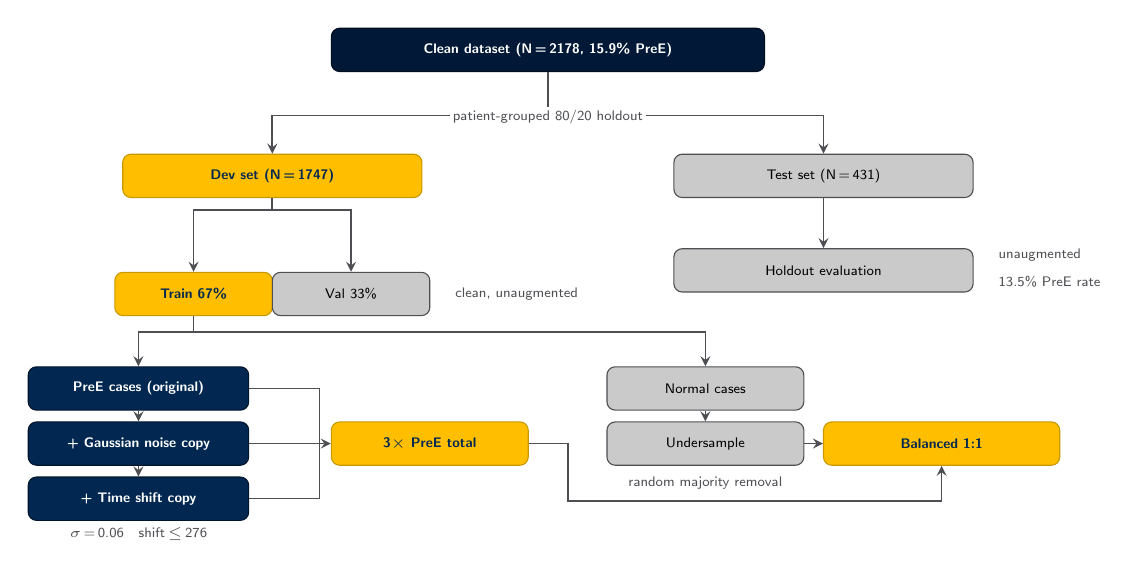
\begin{tikzpicture}[
    x=1cm, y=1cm,
    >=stealth,
    box/.style={
      rectangle, rounded corners=3pt,
      minimum height=0.55cm, minimum width=2.0cm,
      fill=aggieblue, draw=aggieblue!55!black, line width=0.4pt,
      text=white, font=\fontsize{5.5}{6.5}\selectfont\bfseries,
      align=center, inner sep=3pt,
    },
    goldbox/.style={
      rectangle, rounded corners=3pt,
      minimum height=0.55cm, minimum width=2.0cm,
      fill=aggiegold, draw=aggiegoldDark, line width=0.4pt,
      text=aggieblue, font=\fontsize{5.5}{6.5}\selectfont\bfseries,
      align=center, inner sep=3pt,
    },
    graybox/.style={
      rectangle, rounded corners=3pt,
      minimum height=0.55cm,
      fill=coolgray!30, draw=coolgray, line width=0.4pt,
      text=black, font=\fontsize{5}{6}\selectfont,
      align=center, inner sep=3pt,
    },
    darkbox/.style={
      rectangle, rounded corners=3pt,
      minimum height=0.55cm, minimum width=2.0cm,
      fill=aggieblueDark, draw=aggieblueDark!55!black, line width=0.4pt,
      text=white, font=\fontsize{5.5}{6.5}\selectfont\bfseries,
      align=center, inner sep=3pt,
    },
    arr/.style={->, draw=coolgray, line width=0.6pt},
    annot/.style={font=\fontsize{4.5}{5.5}\selectfont, text=coolgray},
    seclab/.style={font=\fontsize{6}{7}\selectfont\bfseries, text=aggieblue},
  ]

  % ---- Full dataset ----
  \node[darkbox, minimum width=5.5cm] (full) at (0, 3.2) {Clean dataset (N\,=\,2178, 15.9\% PreE)};

  % ---- 80/20 patient-grouped holdout ----
  \node[goldbox, minimum width=3.8cm] (dev)  at (-3.5, 1.6) {Dev set (N\,=\,1747)};
  \node[graybox, minimum width=3.8cm] (test) at (3.5, 1.6)  {Test set (N\,=\,431)};

  \draw[arr] (full.south) -- ++(0,-0.55) -| (dev.north);
  \draw[arr] (full.south) -- ++(0,-0.55) -| (test.north);
  \node[annot, fill=white, inner sep=1pt] at (0, 2.35) {patient-grouped 80/20 holdout};

  % ---- Test path (right side) ----
  \node[graybox, minimum width=3.8cm] (testeval) at (3.5, 0.4) {Holdout evaluation};
  \draw[arr] (test) -- (testeval);
  \node[annot, anchor=west] at (5.6, 0.6) {unaugmented};
  \node[annot, anchor=west] at (5.6, 0.25) {13.5\% PreE rate};

  % ---- 3-fold CV on dev (left side) ----
  \node[goldbox, minimum width=2.0cm] (train) at (-4.5, 0.1) {Train 67\%};
  \node[graybox, minimum width=2.0cm] (val)   at (-2.5, 0.1) {Val 33\%};

  \draw[arr] (dev.south) -- ++(0,-0.15) -| (train.north);
  \draw[arr] (dev.south) -- ++(0,-0.15) -| (val.north);
  \node[annot, anchor=west] at (-1.3, 0.1) {clean, unaugmented};

  % ---- Augmentation (train fold only) ----

  % Step 1: PE positive cases get 2 augmented copies appended
  \node[box, minimum width=2.8cm] (pe) at (-5.2, -1.1) {PreE cases (original)};
  \node[box, minimum width=2.8cm] (gn) at (-5.2, -1.8) {+ Gaussian noise copy};
  \node[box, minimum width=2.8cm] (ts) at (-5.2, -2.5) {+ Time shift copy};
  \node[annot] at (-5.2, -2.95) {$\sigma$\,=\,0.06\quad shift\,$\leq$\,276};

  \draw[arr] (train.south) -- ++(0,-0.2) -| (pe.north);
  \draw[arr] (pe) -- (gn);
  \draw[arr] (gn) -- (ts);

  % Step 2: three arrows converge into 3x PE
  \node[goldbox, minimum width=2.5cm] (triple) at (-1.5, -1.8) {3$\times$ PreE total};
  \draw[draw=coolgray, line width=0.5pt] (pe.east) -- (-2.9, -1.1);
  \draw[draw=coolgray, line width=0.5pt] (gn.east) -- (-2.9, -1.8);
  \draw[draw=coolgray, line width=0.5pt] (ts.east) -- (-2.9, -2.5);
  \draw[draw=coolgray, line width=0.5pt] (-2.9, -1.1) -- (-2.9, -2.5);
  \draw[arr]  (-2.9, -1.8) -- (triple.west);

  % Step 3: Normal undersampled
  \node[graybox, minimum width=2.5cm] (norm) at (2.0, -1.1) {Normal cases};
  \draw[arr] (train.south) -- ++(0,-0.2) -| (norm.north);
  \node[graybox, minimum width=2.5cm] (usamp) at (2.0, -1.8) {Undersample};
  \draw[arr] (norm) -- (usamp);
  \node[annot] at (2.0, -2.3) {random majority removal};

  % Step 4: merge to balanced set — 3xPE routes under usamp
  \node[goldbox, minimum width=3.0cm] (bal) at (5.0, -1.8) {Balanced 1:1};
  \draw[arr] (usamp.east) -- (bal.west);
  \draw[arr] (triple.east) -- ++(0.5,0) |- ([yshift=-0.45cm]usamp.south) -| (bal.south);

  \end{tikzpicture}
\end{frame}

% =========================================================
\section{Hyperparameter Optimization}
% =========================================================

\begin{frame}{Stage 1: Learning Rate \& Dropout}
  \begin{columns}[T]
    \begin{column}{0.38\textwidth}
      \small
      \textbf{20 trials} over 1\,h\,34\,m.\\
      Fixed: filters (32,64,128), kernels (7,5,3), 430\,K params.

      \vspace{0.6em}
      \begin{block}{\scriptsize Best Trial \#13}
        \scriptsize
        lr = 0.00247 \quad dropout = 0.055\\[0.15em]
        CV AUROC: \textbf{0.7025}\\
        Test AUROC: \textbf{0.7540}
      \end{block}

      \vspace{0.4em}
      {\footnotesize\color{coolgray}
      Higher learning rates consistently outperformed conservative ones.
      Dropout had minimal impact at this model size.}
    \end{column}
    \begin{column}{0.60\textwidth}
      \centering
      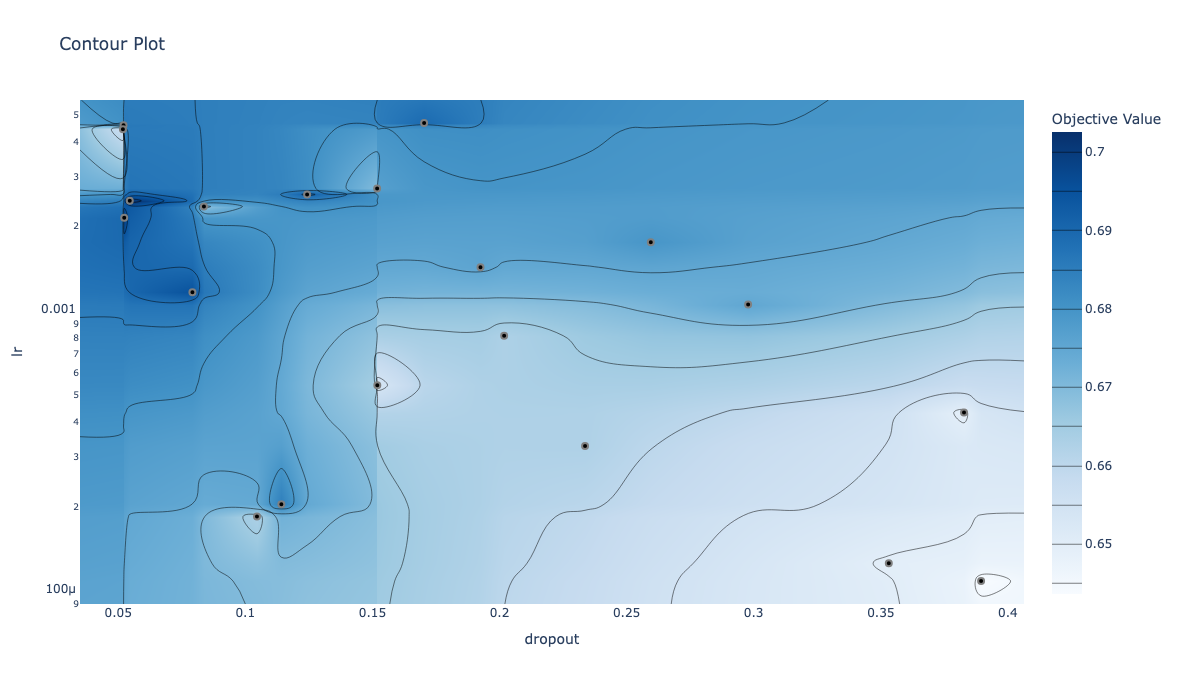
\includegraphics[width=\linewidth]{contour_stage1.png}
    \end{column}
  \end{columns}
\end{frame}

\begin{frame}{Stage 2: Regularization}
  \begin{columns}[T]
    \begin{column}{0.38\textwidth}
      \small
      \textbf{30 trials} over 2\,h\,32\,m.\\
      Fixed from Stage~1: lr, dropout.

      \vspace{0.6em}
      \begin{block}{\scriptsize Best Trial \#20}
        \scriptsize
        wd = 1.67e-4\;\; $\sigma$ = 0.060\;\; shift = 276\\[0.15em]
        CV AUROC: \textbf{0.7032}\;\;{\color{coolgray}($+$0.001)}\\
        Test AUROC: \textbf{0.7219}
      \end{block}

      \vspace{0.4em}
      {\footnotesize\color{coolgray}
      Light weight decay and modest augmentation. Marginal CV gain
      suggests the 430\,K model was not yet capacity-limited ---
      regularization alone cannot overcome underfitting.}
    \end{column}
    \begin{column}{0.60\textwidth}
      \centering
      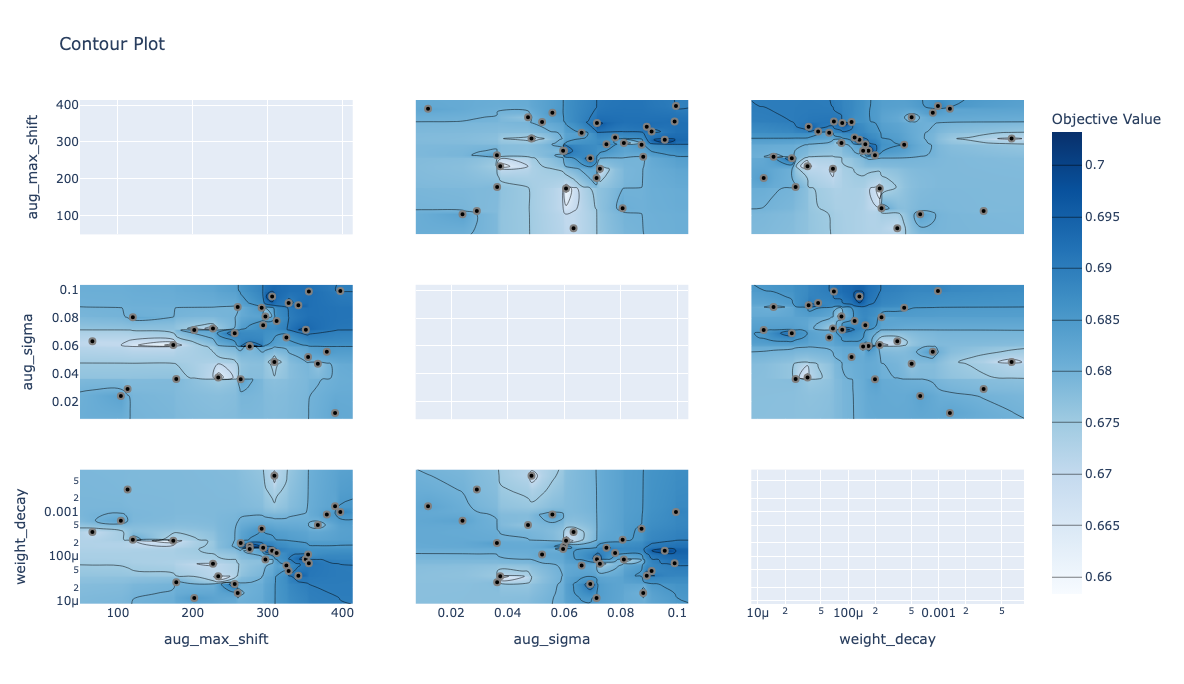
\includegraphics[width=\linewidth]{contour_stage2.png}
    \end{column}
  \end{columns}
\end{frame}

\begin{frame}{Stage 3: Receptive Field (Kernel Sizes)}
  \begin{columns}[T]
    \begin{column}{0.38\textwidth}
      \small
      \textbf{20 trials} over 1\,h\,43\,m.\\
      8 kernel configurations tested (116--356\,ms RF).\\
      Fixed from Stages 1--2: lr, dropout, wd, augmentation.

      \vspace{0.6em}
      \begin{block}{\scriptsize Best Trial \#6}
        \scriptsize
        kernels = (7,\,5,\,3) --- RF = 180\,ms\\[0.15em]
        CV AUROC: \textbf{0.7022}\\
        Test AUROC: \textbf{0.7817}
      \end{block}

      \vspace{0.4em}
      {\footnotesize\color{coolgray}
      Default kernel triple confirmed optimal. The 180\,ms
      receptive field covers the QRS complex --- neither
      sub-QRS nor QT-spanning kernels improved performance.}
    \end{column}
    \begin{column}{0.60\textwidth}
      \centering
      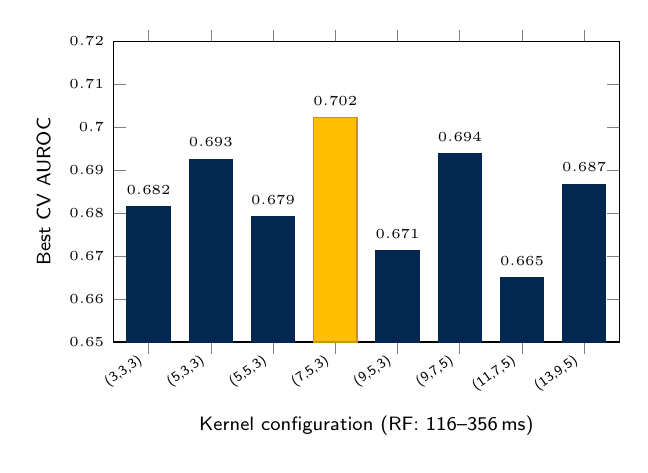
\begin{tikzpicture}
        \begin{axis}[
          repnet base,
          width=8.0cm,
          height=5.4cm,
          ybar,
          bar width=0.55cm,
          symbolic x coords={
            {(3,3,3)},{(5,3,3)},{(5,5,3)},{(7,5,3)},
            {(9,5,3)},{(9,7,5)},{(11,7,5)},{(13,9,5)}},
          xtick=data,
          x tick label style={font=\tiny,rotate=35,anchor=east},
          ylabel={Best CV AUROC},
          ymin=0.65, ymax=0.72,
          ytick={0.65,0.66,0.67,0.68,0.69,0.70,0.71,0.72},
          nodes near coords={\pgfmathprintnumber[fixed,precision=3]{\pgfplotspointmeta}},
          every node near coord/.append style={font=\fontsize{4}{5}\selectfont,above=1pt},
          enlarge x limits=0.08,
          xlabel={Kernel configuration (RF: 116--356\,ms)},
        ]
          \addplot[fill=aggieblue,draw=aggieblue,bar shift=0pt] coordinates {
            ({(3,3,3)},0.6815)
            ({(5,3,3)},0.6925)
            ({(5,5,3)},0.6792)
            ({(7,5,3)},0.7022)
            ({(9,5,3)},0.6712)
            ({(9,7,5)},0.6938)
            ({(11,7,5)},0.6649)
            ({(13,9,5)},0.6867)
          };
          \addplot[fill=aggiegold,draw=aggiegoldDark,bar shift=0pt,
                   nodes near coords style={opacity=0}] coordinates {
            ({(7,5,3)},0.7022)
          };

        \end{axis}
      \end{tikzpicture}
    \end{column}
  \end{columns}
\end{frame}

\begin{frame}{Stage 4: Model Capacity --- The Breakthrough}
  \begin{columns}[T]
    \begin{column}{0.38\textwidth}
      \small
      \textbf{30 trials} over 5\,h\,21\,m.\\
      8 filter configurations (27\,K--965\,K params).\\
      Fixed from Stages 1--3: all prior hyperparameters.

      \vspace{0.6em}
      \begin{block}{\scriptsize Best Trial \#14}
        \scriptsize
        filters = (48,\,96,\,192) --- 965\,K params\\[0.15em]
        CV AUROC: \textbf{0.7034}\\
        Test AUROC: \textbf{0.7952}\;\;{\color{aggiegoldDark}($+$4.1\%)}
      \end{block}

      \vspace{0.4em}
      {\footnotesize\color{coolgray}
      The largest model won decisively on test AUROC despite modest
      CV gains. Confirmed the bottleneck was model capacity, not
      regularization or receptive field.}
    \end{column}
    \begin{column}{0.60\textwidth}
      \centering
      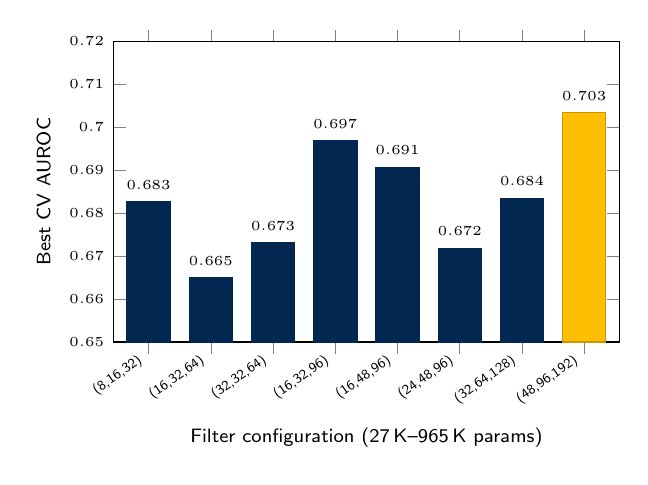
\begin{tikzpicture}
        \begin{axis}[
          repnet base,
          width=8.0cm,
          height=5.4cm,
          ybar,
          bar width=0.55cm,
          symbolic x coords={
            {(8,16,32)},{(16,32,64)},{(32,32,64)},{(16,32,96)},
            {(16,48,96)},{(24,48,96)},{(32,64,128)},{(48,96,192)}},
          xtick=data,
          x tick label style={font=\tiny,rotate=35,anchor=east},
          ylabel={Best CV AUROC},
          ymin=0.65, ymax=0.72,
          ytick={0.65,0.66,0.67,0.68,0.69,0.70,0.71,0.72},
          nodes near coords={\pgfmathprintnumber[fixed,precision=3]{\pgfplotspointmeta}},
          every node near coord/.append style={font=\fontsize{4}{5}\selectfont,above=1pt},
          enlarge x limits=0.08,
          xlabel={Filter configuration (27\,K--965\,K params)},
        ]
          \addplot[fill=aggieblue,draw=aggieblue,bar shift=0pt] coordinates {
            ({(8,16,32)},0.6826)
            ({(16,32,64)},0.6650)
            ({(32,32,64)},0.6731)
            ({(16,32,96)},0.6969)
            ({(16,48,96)},0.6907)
            ({(24,48,96)},0.6718)
            ({(32,64,128)},0.6835)
            ({(48,96,192)},0.7034)
          };
          \addplot[fill=aggiegold,draw=aggiegoldDark,bar shift=0pt,
                   nodes near coords style={opacity=0}] coordinates {
            ({(48,96,192)},0.7034)
          };

        \end{axis}
      \end{tikzpicture}
    \end{column}
  \end{columns}
\end{frame}

% =========================================================
\section{Best Model Analysis}
% =========================================================

\begin{frame}{Test Set ROC \& Score Distribution}
  \begin{columns}[T]
    \begin{column}{0.50\textwidth}
      \centering
      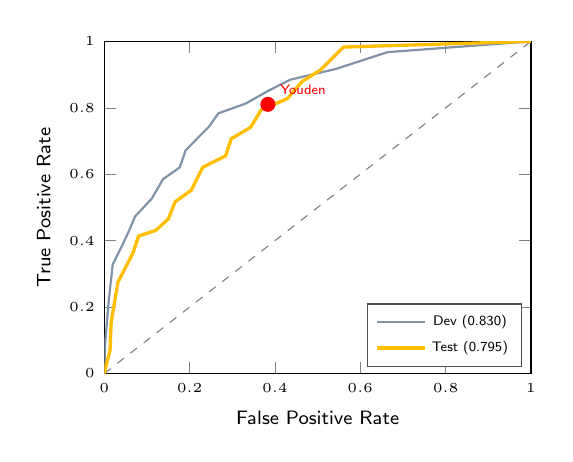
\begin{tikzpicture}
        \begin{axis}[
          repnet base,
          width=7.0cm,
          height=5.8cm,
          xlabel={False Positive Rate},
          ylabel={True Positive Rate},
          xmin=0, xmax=1, ymin=0, ymax=1,
          xtick={0,0.2,0.4,0.6,0.8,1.0},
          ytick={0,0.2,0.4,0.6,0.8,1.0},
          legend style={at={(0.98,0.02)},anchor=south east,
                        font=\tiny,draw=coolgray,fill=white},
        ]
          % Diagonal reference
          \addplot[gray,dashed,thin,forget plot] coordinates {(0,0)(1,1)};

          % Dev ROC
          \addplot[aggieblue!50,thick] coordinates {
            (0.0000,0.0000)
            (0.0020,0.0903)
            (0.0102,0.2166)
            (0.0197,0.3285)
            (0.0395,0.3791)
            (0.0605,0.4368)
            (0.0721,0.4729)
            (0.1116,0.5271)
            (0.1374,0.5848)
            (0.1769,0.6209)
            (0.1905,0.6715)
            (0.2177,0.7076)
            (0.2456,0.7437)
            (0.2673,0.7834)
            (0.3306,0.8123)
            (0.3857,0.8520)
            (0.4354,0.8845)
            (0.5429,0.9170)
            (0.6639,0.9675)
            (1.0000,1.0000)
          };
          \addlegendentry{Dev (0.830)}

          % Test ROC
          \addplot[aggiegold,very thick] coordinates {
            (0.0000,0.0000)
            (0.0027,0.0172)
            (0.0134,0.0690)
            (0.0161,0.1552)
            (0.0322,0.2759)
            (0.0670,0.3621)
            (0.0804,0.4138)
            (0.1206,0.4310)
            (0.1501,0.4655)
            (0.1662,0.5172)
            (0.2038,0.5517)
            (0.2306,0.6207)
            (0.2842,0.6552)
            (0.2976,0.7069)
            (0.3432,0.7414)
            (0.3673,0.7931)
            (0.4290,0.8276)
            (0.4638,0.8793)
            (0.5067,0.9138)
            (0.5603,0.9828)
            (1.0000,1.0000)
          };
          \addlegendentry{Test (0.795)}

          % Youden point
          \addplot[only marks,mark=*,mark size=2.5pt,red] coordinates {
            (0.3834,0.8103)
          };
          \node[font=\tiny,anchor=south west,red] at (axis cs:0.39,0.81) {Youden};

        \end{axis}
      \end{tikzpicture}

      {\scriptsize AUROC: Dev\,=\,0.830\quad Test\,=\,0.795\quad Gap\,=\,+0.034}
    \end{column}
    \begin{column}{0.50\textwidth}
      \centering
      {\scriptsize\bfseries P(PreE) score distribution — Test set (N\,=\,431)}\\[0.3em]
      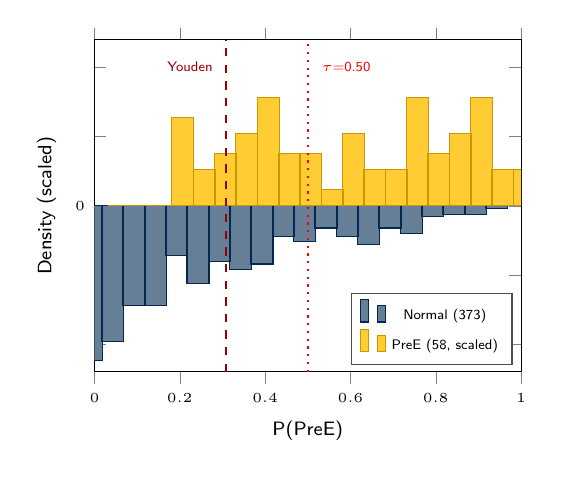
\begin{tikzpicture}
        \begin{axis}[
          repnet base,
          width=7.0cm,
          height=5.8cm,
          ybar,
          bar width=0.28cm,
          xlabel={P(PreE)},
          ylabel={Density (scaled)},
          xmin=0, xmax=1,
          ymin=-60, ymax=60,
          xtick={0,0.2,0.4,0.6,0.8,1.0},
          ytick={-50,-25,0,25,50},
          yticklabels={,,,,},
          extra y tick style={grid=major,grid style={black,thin}},
          extra y ticks={0},
          legend style={at={(0.98,0.02)},anchor=south east,
                        font=\tiny,draw=coolgray,fill=white},
        ]
          % Normal (mirrored below zero) — raw counts
          \addplot[fill=aggieblue!60,draw=aggieblue] coordinates {
            (0.025,-56) (0.075,-49) (0.125,-36) (0.175,-36)
            (0.225,-18) (0.275,-28) (0.325,-20) (0.375,-23)
            (0.425,-21) (0.475,-11) (0.525,-13) (0.575,-8)
            (0.625,-11) (0.675,-14) (0.725,-8) (0.775,-10)
            (0.825,-4) (0.875,-3) (0.925,-3) (0.975,-1)
          };
          \addlegendentry{Normal (373)}

          % PreE (above zero) — scaled by 373/58 = 6.43 so heights are comparable
          \addplot[fill=aggiegold!80,draw=aggiegoldDark] coordinates {
            (0.025,0) (0.075,0) (0.125,0) (0.175,32)
            (0.225,13) (0.275,19) (0.325,26) (0.375,39)
            (0.425,19) (0.475,19) (0.525,6) (0.575,26)
            (0.625,13) (0.675,13) (0.725,39) (0.775,19)
            (0.825,26) (0.875,39) (0.925,13) (0.975,13)
          };
          \addlegendentry{PreE (58, scaled)}

          % Threshold lines
          \draw[red,dotted,thick] (axis cs:0.5,-60) -- (axis cs:0.5,60);
          \node[font=\tiny,red,anchor=south west] at (axis cs:0.51,45) {$\tau$=0.50};

          \draw[red!60!black,dashed,thick] (axis cs:0.308,-60) -- (axis cs:0.308,60);
          \node[font=\tiny,red!60!black,anchor=south east] at (axis cs:0.30,45) {Youden};
        \end{axis}
      \end{tikzpicture}

      {\scriptsize PreE $\uparrow$ \quad Normal $\downarrow$ \quad Dashed\,=\,$\tau$\,=\,0.50}
    \end{column}
  \end{columns}
\end{frame}

\begin{frame}{Classification Report --- Test Set}
  \begin{columns}[T]
    \begin{column}{0.52\textwidth}
      \centering
      {\small\bfseries Per-class metrics (N\,=\,431: 373 Normal, 58 PreE)}\\[0.5em]
      \renewcommand{\arraystretch}{1.3}
      \footnotesize
      \begin{tabular}{@{}l cc cc@{}}
        \toprule
        & \multicolumn{2}{c}{\bfseries $\tau$\,=\,0.50} &
          \multicolumn{2}{c}{\bfseries $\tau$\,=\,0.31} \\
        &  \multicolumn{2}{c}{\scriptsize(default)} &
           \multicolumn{2}{c}{\scriptsize(Youden's J)} \\
        \cmidrule(lr){2-3} \cmidrule(lr){4-5}
        \textbf{Metric} & \textbf{Normal} & \textbf{PreE}
                         & \textbf{Normal} & \textbf{PreE} \\
        \midrule
        Precision  & 0.92 & 0.30 & 0.96 & 0.25 \\
        Recall     & 0.80 & 0.55 & 0.62 & 0.83 \\
        F1-score   & 0.86 & 0.39 & 0.75 & 0.39 \\
        \midrule
        Accuracy   & \multicolumn{2}{c}{0.77} & \multicolumn{2}{c}{0.65} \\
        \bottomrule
      \end{tabular}

      \vspace{0.8em}
      {\small\bfseries Clinical screening metrics}\\[0.3em]
      \footnotesize
      \begin{tabular}{@{}l cccc@{}}
        \toprule
        & \textbf{Sensitivity} & \textbf{Specificity} & \textbf{PPV} & \textbf{NPV} \\
        \midrule
        $\tau$\,=\,0.50 & 0.552 & 0.799 & 0.299 & 0.920 \\
        $\tau$\,=\,0.31 & \textbf{0.828} & 0.617 & 0.251 & \textbf{0.958} \\
        \bottomrule
      \end{tabular}
    \end{column}
    \begin{column}{0.46\textwidth}
      \small
      \begin{block}{\scriptsize Threshold trade-off}
        \scriptsize
        \textbf{$\tau$\,=\,0.50} balances precision and recall.\\
        Catches 55\% of PreE cases; 30\% of positive predictions are correct.\\[0.4em]
        \textbf{$\tau$\,=\,0.31} (Youden's J) maximizes sensitivity + specificity.\\
        Catches 83\% of PreE; only misses 10/58 cases.\\
        NPV\,=\,0.958: a negative screen is highly reliable.
      \end{block}

      \vspace{0.4em}
      \begin{block}{\scriptsize Generalization}
        \scriptsize
        AUROC gap: 0.830 (dev) $\to$ 0.795 (test) = +0.034\\[0.2em]
        Modest gap suggests the model generalizes well and is not
        overfitting to the training distribution despite class imbalance
        (13.5\% PreE prevalence in test).
      \end{block}

      \vspace{0.4em}
      {\footnotesize\color{coolgray}
      For a screening tool, the Youden threshold is preferred:
      high sensitivity minimizes missed diagnoses at the cost
      of more follow-up confirmations.}
    \end{column}
  \end{columns}
\end{frame}

\begin{frame}{Confusion Matrices --- Threshold Comparison}
  \begin{columns}[T]
    \begin{column}{0.48\textwidth}
      \centering
      {\small\bfseries $\tau$\,=\,0.50 (default threshold)}\\[0.4em]
      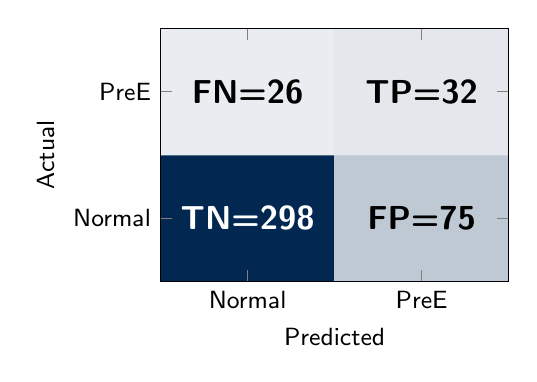
\begin{tikzpicture}
        \begin{axis}[
          width=6.0cm, height=4.8cm,
          colormap={blues}{color(0)=(white) color(1)=(aggieblue)},
          xmin=-0.5, xmax=1.5, ymin=-0.5, ymax=1.5,
          xtick={0,1}, xticklabels={Normal,PreE},
          ytick={0,1}, yticklabels={PreE,Normal},
          xlabel={Predicted},
          ylabel={Actual},
          tick label style={font=\small},
          label style={font=\small},
          point meta min=0, point meta max=300,
          enlargelimits=false,
          axis on top,
        ]
          \addplot[matrix plot, point meta=explicit,
                   mesh/cols=2, mesh/rows=2] coordinates {
            (0,1) [298]  (1,1) [75]
            (0,0) [26]   (1,0) [32]
          };
          \node[font=\large\bfseries,white] at (axis cs:0,1) {TN=298};
          \node[font=\large\bfseries] at (axis cs:1,1) {FP=75};
          \node[font=\large\bfseries] at (axis cs:0,0) {FN=26};
          \node[font=\large\bfseries] at (axis cs:1,0) {TP=32};
        \end{axis}
      \end{tikzpicture}

      \vspace{0.3em}
      {\footnotesize
      \begin{tabular}{@{}ll@{}}
        Sensitivity: & 32/58 = \textbf{55.2\%} \\
        Specificity: & 298/373 = \textbf{79.9\%} \\
        Accuracy:    & 330/431 = \textbf{76.6\%} \\
      \end{tabular}}

      \vspace{0.4em}
      {\scriptsize\color{coolgray}
      Misses 26 PreE cases (44.8\% false negatives).\\
      Conservative: fewer false alarms, more missed diagnoses.}
    \end{column}
    \begin{column}{0.48\textwidth}
      \centering
      {\small\bfseries $\tau$\,=\,0.31 (Youden's J)}\\[0.4em]
      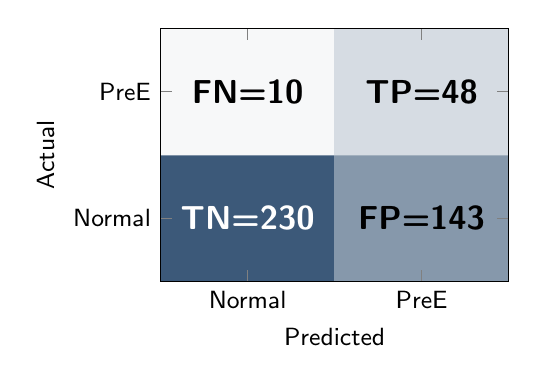
\begin{tikzpicture}
        \begin{axis}[
          width=6.0cm, height=4.8cm,
          colormap={blues}{color(0)=(white) color(1)=(aggieblue)},
          xmin=-0.5, xmax=1.5, ymin=-0.5, ymax=1.5,
          xtick={0,1}, xticklabels={Normal,PreE},
          ytick={0,1}, yticklabels={PreE,Normal},
          xlabel={Predicted},
          ylabel={Actual},
          tick label style={font=\small},
          label style={font=\small},
          point meta min=0, point meta max=300,
          enlargelimits=false,
          axis on top,
        ]
          \addplot[matrix plot, point meta=explicit,
                   mesh/cols=2, mesh/rows=2] coordinates {
            (0,1) [230]  (1,1) [143]
            (0,0) [10]   (1,0) [48]
          };
          \node[font=\large\bfseries,white] at (axis cs:0,1) {TN=230};
          \node[font=\large\bfseries] at (axis cs:1,1) {FP=143};
          \node[font=\large\bfseries] at (axis cs:0,0) {FN=10};
          \node[font=\large\bfseries] at (axis cs:1,0) {TP=48};
        \end{axis}
      \end{tikzpicture}

      \vspace{0.3em}
      {\footnotesize
      \begin{tabular}{@{}ll@{}}
        Sensitivity: & 48/58 = \textbf{82.8\%} \\
        Specificity: & 230/373 = \textbf{61.7\%} \\
        Accuracy:    & 278/431 = \textbf{64.5\%} \\
      \end{tabular}}

      \vspace{0.4em}
      {\scriptsize\color{coolgray}
      Only misses 10 PreE cases (17.2\% false negatives).\\
      Preferred for screening: catches most positives.}
    \end{column}
  \end{columns}
\end{frame}

% =========================================================
\section{Model Interpretability}
% =========================================================

\begin{frame}{Cross-Lead Attention \& Lead Importance}
  \centering
  
\includegraphics[width=\linewidth,height=0.70\textheight,keepaspectratio]{fig_attention.pdf}

  \vspace{0.2em}
  {\scriptsize
  \textbf{Left:} Mean attention weights per stage (rows\,=\,query, cols\,=\,key).
  Blue\,=\,Normal, Red\,=\,PreE.
  \quad\textbf{Right:} Stage\,3 $\Delta$attention (PreE$-$Normal) --- leads the model
  attends to more for PreE.}
\end{frame}

\begin{frame}{Saliency --- Top 6 Leads (Strongest Attribution)}
  \centering
  
\includegraphics[width=\linewidth,height=0.70\textheight,keepaspectratio]{fig_saliency_1.pdf}

  \vspace{0.2em}
  {\scriptsize
  Confident PreE case (P(PreE)\,=\,0.965). Combined IG\,+\,Grad-CAM, log-scaled.
  \textcolor{red}{\textbf{Red}}\,=\,pushes toward PreE,
  \textcolor{blue}{\textbf{blue}}\,=\,pushes toward Normal.
  Leads ordered by total attribution magnitude.}
\end{frame}

\begin{frame}{Saliency --- Remaining 6 Leads}
  \centering
  
\includegraphics[width=\linewidth,height=0.70\textheight,keepaspectratio]{fig_saliency_2.pdf}

  \vspace{0.2em}
  {\scriptsize
  Same case continued. Lower-ranked leads show weaker but still structured attribution,
  confirming the model uses cross-lead information rather than relying on a single lead.}
\end{frame}

\begin{frame}{Activation Propagation --- Stage 1}
  \centering
  
\includegraphics[width=\linewidth,height=0.70\textheight,keepaspectratio]{fig_activations_1.pdf}

  \vspace{0.3em}
  {\scriptsize
  48 filters (k\,=\,7, 28\,ms) detect local waveform shapes.
  Attention gates outputs using cross-lead context. Resolution: 2500\,$\to$\,1250.}
\end{frame}

\begin{frame}{Activation Propagation --- Stage 2}
  \centering
  
\includegraphics[width=\linewidth,height=0.70\textheight,keepaspectratio]{fig_activations_2.pdf}

  \vspace{0.3em}
  {\scriptsize
  96 filters (k\,=\,5) capture ST-segment and T-wave morphology.
  Attention sharpens channels via cross-lead agreement. Resolution: 1250\,$\to$\,625.}
\end{frame}

\begin{frame}{Activation Propagation --- Stage 3}
  \centering
  
\includegraphics[width=\linewidth,height=0.70\textheight,keepaspectratio]{fig_activations_3.pdf}

  \vspace{0.3em}
  {\scriptsize
  192 filters (k\,=\,3) at coarsest resolution (625\,$\to$\,312).
  Highest-level features spanning 180\,ms. Fused across leads, then pooled for classification.}
\end{frame}

\begin{frame}{Feature Voting --- Fusion to Classification}
  \centering
  
\includegraphics[width=\linewidth,height=0.70\textheight,keepaspectratio]{fig_activations_vote.pdf}

  \vspace{0.3em}
  {\scriptsize
  1$\times$1 conv projects 2304 (12$\times$192) lead-channels\,$\to$\,192 features per timestep.
  GAP averages over time\,$\to$\,192-dim vector.
  Each channel votes via activation\,$\times$\,weight; the sum determines the prediction.}
\end{frame}

% =========================================================
\section*{Acknowledgements}
% =========================================================

{%
  \setbeamertemplate{footline}{}%
  \begin{frame}[plain,noframenumbering]
    \begin{tikzpicture}[remember picture,overlay]
      \fill[aggieblue] (current page.south west) rectangle (current page.north east);
    \end{tikzpicture}
    \vfill
    \centering
    {\Raleway\bfseries\Huge\color{white} Thank you}\\[0.6em]
    {\color{aggiegold}\rule{4cm}{0.06cm}}\\[0.8em]
    {\Lato\large\color{white} Questions?}
    \vfill
  \end{frame}
}

\end{document}
